\documentclass[a4paper, titlepage]{report}

\usepackage[a4paper]{geometry}
\geometry{verbose, tmargin=2.0cm, bmargin=2.0cm, lmargin=2.0cm, rmargin=2.0cm}

%hyper references pdf attributes
\usepackage{hyperref}
\hypersetup{
pdftitle={Hello Window!},
pdfauthor={Szilárd Pfeiffer},
pdfsubject={GTK+ and gtkmm programming},
pdfkeywords={szilárd pfeiffer, gtk, gtk+, gtkmm, gnome, hig, linux},
bookmarks={true},
unicode={true},
colorlinks={false},
hyperfigures={true},
a4paper={true}
}

\input{common_preamble}

\author{
\href{http://pfeifferszilard.hu}{Szilárd Pfeiffer}
}
\title{Hello Window!}

\begin{document}

\maketitle

\pagenumbering{roman}
\tableofcontents
\newpage
\pagenumbering{arabic}

\chapter{Bevezetés}

\section{Bevezetés}
\index{GtkWindow@\texttt{GtkWindow}}
\index{GtkDialog@\texttt{GtkDialog}}

Ebben a részében a \textit{GTK}-ban létrehozható különböző ablaktípusok közös vonásait, valamint eltéréseit, illetve ezek okait vesszük sorra. Kitérünk egyrészről az egyes ablaktípusok létrehozásának sajátosságaira, azok \textit{widget}ekkel való feltöltésére, másrészről a felhasználó interakciók kezelésére, ezzel együtt az ablakok bezárásának módjaira is, szem előtt tartva természetese a \textit{C}, \textit{C++}, illetve \textit{Python} nyelvű változat azonosságait, különbözőségeit.

\subsection{\textit{Popup} és \textit{toplevel} ablakok}
\label{sec:windowtype}
\index{ablak!típus!popup}
\index{ablak!típus!toplevel}
\index{GtkWindow@\texttt{GtkWindow}!tulajdonságok!type@\texttt{type}}

A \textit{popup} ablakra, mint típusra ugyan ritkán lesz közvetlenül szükségünk, érdemes tudni, hogy a \textit{GTK} ebben a tekintetben két fajta ablakot különböztet meg. A \textit{popup} (felugró, felbukkanó) ablakokat, melyekre -- valamilyen speciális célt szolgáló saját készítésű \textit{widget}ektől eltekintve -- csak néhány példa létezik (\textit{menu}, \textit{tooltip}), valamint a \textit{toplevel} (legkülső, legfelső szintű) ablakokat, melyek csaknem minden \textit{GTK}-s, illetve saját fejlesztésű ablak alapjául szolgálnak. Ha tehát az ablakra, illetve a hozzá kapcsolódó fogalmakra gondolunk, többségében egy \textit{toplevel} ablakra gondolunk, és nem a \textit{popup}\footnote{Más eszközkészletek a ``popups'' gyűjtőfogalom alá sorolják a dialógusokat, a \textit{GTK} esetén azonban egy dialógus ablak mindig egy \textit{toplevel}} típusúakra, melyekről talán nem is feltételeznénk első ránézésre, hogy ablakok.

\index{GtkWindow@\texttt{GtkWindow}!tulajdonságok!type@\texttt{type}}
Az ablakkezelő ezt az információt használja fel annak eldöntésére, hogy az adott ablakot milyen kerettel, dekorációval lássa el, illetve hogy általánosságban menedzselje e ablakot. Utóbbi -- azaz a \textit{toplevel} ablakok -- esetben alapértelmezetten az ablakkezelő keretet, illetve a beállításoktól függően azon például bezáró, teljes mértre váltó, minimalizáló gombot jelenít meg. A \textit{popup} típusú ablakokat az ablakkezelő nemcsak hogy nem dekorálja, de nem is menedzseli azokat, következésképp tehát számos -- az ablakkezelő hatáskörébe tartozó -- funkció, mint amilyen például a minimalizálás, vagy a maximalizálás nem is érhető el. Bár kézenfekvő megoldásnak látszik a \textit{popup} típus arra, ha egy dekoráció nélküli ablakot készítsünk, mégse ezt tegyük, az ilyen típusú megjelenésbeli sajátosságok beállítására léteznek külön függvények.

\index{GtkBin@\texttt{GtkBin}}
Minden \texttt{GtkWindow} egyben konténer is, pontosabban fogalmazva egy \textit{GtkBin}, azaz tartalmazhat egy további elemet gyerekként, ami természetesen szintén lehet egy konténer, így biztosítva, hogy számos elemet helyezhessünk el az elkészített ablakon belül.

\subsection{\textit{Window} és \textit{dialóg}}
\index{GtkWindow@\texttt{GtkWindow}}
\index{GtkDialog@\texttt{GtkDialog}}
\index{GtkBox@\texttt{GtkBox}!függvények!pack\_end@\texttt{pack\_end}}
\index{GtkBox@\texttt{GtkBox}!függvények!pack\_start@\texttt{pack\_start}}

\label{par:dialogbox}
\index{ablak!típus!toplevel}
\index{GtkBox@\texttt{GtkBox}}
\index{GtkButtonBox@\texttt{GtkButtonBox}}
\index{GtkSeparator@\texttt{GtkSeparator}}
\index{GtkDialog@\texttt{GtkDialog}!belső elemek!action\_area@\texttt{action\_area}}
\index{GtkBox@\texttt{GtkBox}!függvények!pack\_start@\texttt{pack\_start}}
\index{GtkBox@\texttt{GtkBox}!függvények!pack\_end@\texttt{pack\_end}}
A \textit{window} típus -- azon belül is ahogy tárgyaltuk a \textit{toplevel window} -- közvetlen szülője a \textit{dialog} típusnak, számottevő különbség tulajdonképpen nincs is a kettő között. Egy \textit{dialog} nem más, mint egy olyan \textit{window}, melybe a \textit{GTK+} fejlesztői néhány hasznos elemet helyeztek el. Konkrétabban fogalmazva minden dialógba egy függőleges elrendezésű konténer \textit{widget} (\texttt{GtkBox}), abba pedig egy, a gombok elhelyezésére szolgáló konténer (\texttt{GtkButtonBox} típusú \texttt{action\_area}), valamint egy szeparátor (\texttt{GtkSeparator}) kerül, ebben a sorrendben mindkét esetben a konténer aljára helyezve\footnote{A \texttt{GtkBox} típus \texttt{pack\_end()} függvényét hívva.}. Ebből következik, hogy minden, amit egy dialógusba -- annak elkészült után -- tenni akarunk az a gombsor, valamint a vízszintes szeparátor fölött jelenik meg, függetlenül attól, hogy azt a \texttt{pack\_start()}, vagy a \texttt{pack\_end()} függvény segítségével helyezzük el a konténerben.

\index{GtkDialog@\texttt{GtkDialog}!belső elemek!content\_area@\texttt{content\_area}}
A \textit{dialog} típus tehát -- a szeparátor által -- függőlegesen ketté osztott \textit{window}, ahol az alsó rész (\texttt{action\_area}), ami általában a gombokat tartalmazza (pl.: Ok, Mégse, Súgó, \dots), a felső (\texttt{content\_area}) pedig azokat az elemeket tartalmazza, amik a felhasználói számára a szükséges akcióhoz (pl.: adatbevitel, hibaüzenet megjelenítése, \dots) szükséges.

\subsection{Modalitás}
\label{sec:windowmodal}

\index{ablak!modalitás}
\index{GtkWindow@\texttt{GtkWindow}!tulajdonságok!modal@\texttt{modal}}
A több ablakkal történő párhuzamos interakció tiltására szolgál a \textit{window} \textit{modal} tulajdonsága. Amennyiben egy ablak ``modális'' csak az abban az ablakban elhelyezkedő \textit{widget}ekbe történhet például bevitel, csak azokon váltódhat ki valamilyen felhasználó által kezdeményezett esemény. Ezt kihasználva biztosíthatjuk például, hogy egy adatbeviteli ablak\footnote{Ilyen lehet például a \textit{szerkesztés} menüpontok \textit{beállítások} almenüjének hatására megjelenő ablak.} bezárásáig ne változzon semmilyen, a felhasználó által módosítható, \textit{widget} tartalma a háttérben.

Modalitásnak két formáját különböztetjük meg. Egyrészről -- amiről eddig is szó esett -- a csak az applikációra vonatkozó modalitást, mely lehetővé teszi, hogy más applikációk ablakaihoz minden további nélkül hozzáférhetünk. Másrészről a teljes rendszerre érvényes modalitást, ahol a modális ablakon kívüli ablakokkal folytatott minden nemű felhasználó interakció tiltott. Ez utóbbi módszert csak a legszükségesebb esetben -- már ha van ilyen -- célszerű alkalmazni és az előbbi is csak akkor fogadható el felülettervezési szempontból, ha az applikáció egyéb részeihez való hozzáférés adatvesztést, vagy más komoly hibát okozna. Amennyiben mégis a modalitás mellett döntünk, ami nem ritka, hiszen az adatbevitelre, módosításra használt ablakok majd mindegyike ilyen, fontos egyértelművé tenni a felhasználó számára, hogy miként hagyhatja el azt az ablakot, ami korlátozza az applikáció más részeihez való hozzáférését. Egy ilyen menekülő útvonal biztosításának kézenfekvő módja lehet például egy \textit{Mégse} feliratú gomb.

\subsection{Tranziencia}
\label{sec:windowtransientfor}

\index{ablak!tranziencia}\index{GtkWindow@\texttt{GtkWindow}!tulajdonságok!transient-for@\texttt{transient-for}}
A dialógusok rendszerint ``tranziensek'' arra az ablakra, melyből származnak, azaz arra az ablakra melyen azt a műveletet váltottuk ki, aminek hatására a dialógus megjelent. Ezen beállítás alapján az ablakkezelő képes a dialógusunkat előtérben, a szülőablak fölött tartani\footnote{Helytelen beállítások esetén -- ha rosszul, vagy egyáltalán nem adjuk meg a szülőablakot -- előfordulhat, hogy egy újonnan létrehozott és megjelenített dialógusunk a már létező ablakok alatt, vagy között kerül megjelenítésre, ami felhasználói szempontból roppant zavaró}, valamint ha arra kérjük, akkor a szülő ablakhoz képest középen megjeleníteni (\ref{sec:windowpos}).

\index{GtkWindow@\texttt{GtkWindow}!tulajdonságok!destroy-with-parent@\texttt{destroy-with-parent}}
Ez a funkció azonban nem csak az ablakok helyes megjelenítéséhez szükséges, a megszüntetésükkor is hasznos, hiszen a \texttt{destroy-with-parent} tulajdonságon (\textit{property}) keresztül lehetőség van arra utasítani a \textit{GTK}-t, hogy egy ablak megszűnésekor azokat az ablakokat is szüntesse meg, melyek erre a szülőablakra nézve tranziensek. Ez leginkább akkor hasznos, hogy ha egy bizonytalan ideig létező ablakra szeretnénk tranziensek lenni\footnote{Erre lehet példa egy nem modális ablak, ami a programfutása során is megszűnhet}. Így nem kell törődnünk azzal, hogy ablakaink esetleg ``árván'' maradnak.\label{par:windowdestroywithparent}

\section{Használat}

\subsection{Létrehozás}
\index{GtkWindow@\texttt{GtkWindow}}
\index{GtkDialog@\texttt{GtkDialog}}

Mind a \texttt{GtkDialog}, mind pedig a \texttt{GtkWindow} típus létrehozása -- már ami formai részt illeti --, teljesen hasonló az összes többi \textit{widget}éhez, van azonban egy érdemi különbség, amire érdemes kitérni. Az ablakok -- igaz ez természetesen az összes többi \texttt{GtkWindow} típusból származó \textit{widget}re is (pl.: \texttt{GtkMessageDialog}, \texttt{GtkAboutDialog}, \dots) -- természetüknél fogva nem kerülnek bele más konténerbe, hiszen pont ezek azok a típusok, amik \textit{widget}eket tartalmaznak. Ellentétben azonban a többi típussal, ahol a referenciaszámlálás megoldja a problémát, itt a létrejött \textit{widget}ek felszabadításáról magunknak kell gondoskodnunk.

\subsubsection{Paraméterek}

A \texttt{GtkDialog} létrehozásában már valamivel nagyobb a különbség, függően attól, hogy \textit{GTK+}-t, vagy \textit{gtkmm}et használunk, bár így sem számottevő. Minkét esetben meg kell adnunk a címsor szövegét, valamint azt az ablakot, amire tranziensek kívánunk lenni. \textit{GTK+} esetén -- ahogy látszik -- lehetőségünk van \texttt{NULL} érték megadására, ami azt jelenti, hogy nem kívánunk ezzel a lehetőséggel élni. A \textit{gtkmm} is lehetséges ez, ha az alább látható konstruktort helyett azt hívjuk, amelyből hiányzik a \texttt{parent} paraméter.

\lsttriplesourcev
{sources/window_create.h}
{sources/window_create.hpp}
{sources/window_create.py}
{\textit{Window} létrehozása}
{lst:windowcreate}

\index{ablak!típus}
\index{ablak!típus!popup}
\index{ablak!típus!toplevel}
Ahogy arról szó esett (\ref{sec:windowtype}) a \textit{GTK} két típust különböztet meg -- a \textit{popup} és \textit{toplevel} \textit{window} -- melyek közül az előbbi olyannyira ritkán használt, hogy a \textit{C++} nyelvű változat esetén az alapértelmezett paramétere is van a típus konstruktorának, ahol a típus alapértelmezett értéke \textit{toplevel}.

\index{GtkWindow@\texttt{GtkWindow}!tulajdonságok!modal@\texttt{modal}}
A \textit{C}, illetve a \textit{Python} változat \texttt{flags} paramétere egyben tartalmazza a \textit{gtkmm} \texttt{modal} (\ref{sec:windowmodal}) és a \texttt{destroy-with-parent} (\ref{par:windowdestroywithparent}) értéket egy \textit{bitmask} értékben. Ez utóbbi beállítására ugyan van lehetőség \textit{gtkmm} esetén is, a \textit{C++} nyelvi eszközeinek korrekt használata mellett nemigen van szükség\footnote{Ha egy ablakra egy tranziens dialógust akarunk megjeleníteni, az nyugodtan lehet adattag, aminek megszüntetéséről az ablak destruktorában gondoskodhatunk.}.

\lsttriplesource
[numbers=none]
{sources/dialog_create.h}
{sources/dialog_create.hpp}
{sources/dialog_create.py}
{\textit{Dialog} létrehozása}
{lst:dialogcreate}

\subsubsection{Pozíció}
\label{sec:windowpos}
\index{ablak!pozíció}

Egy ablak képernyőn elfoglalt pozíciójának megadására alapvetően két lehetőség kínálkozik. Az egyik, ha előre -- még az ablak megjelenítése előtt -- megadjuk, a kívánt elhelyezkedést. Ehhez a \textit{GTK} annyiban tud segítségünkre lenni, hogy választhatunk néhány előre definiált elhelyezkedési pozíció közül, így nem szükséges a pixelben megadott koordináták kiszámítására időt és energiát pazarolni\footnote{Ami nem minden esetben kézenfekvő feladat, hiszen adott esetben nem csak a képernyő felbontásával, saját ablakunk méreteivel, de a szülőablak, vagy éppen a desktop szélesség és magasság értékeivel is foglalkozni kell.}.

\index{GtkWindow@\texttt{GtkWindow}!függvények!set\_position@\texttt{set\_position}}
\index{GtkDialog@\texttt{GtkDialog}!függvények!run@\texttt{run}}
\index{GtkWidget@\texttt{GtkWidget}!függvények!show@\texttt{show}}
A \texttt{set\_position} függvény még a megjelenítést megelőzően -- azaz \textit{window} esetén a \texttt{show}, \textit{daialog} esetén pedig a \texttt{run} meghívása előtt -- módunkban áll az alábbi elhelyezkedési sémák közül a megfelelőt kiválasztani.

\begin{description}
 \index{Gtk@\texttt{Gtk}!konstansok!WIN\_POS\_NONE@\texttt{WIN\_POS\_NONE}}
 \item[\texttt{WIN\_POS\_NONE}] Nincs befolyással a megjelenítést ablak pozíciójára nincs.

 \index{Gtk@\texttt{Gtk}!konstansok!WIN\_POS\_CENTER@\texttt{WIN\_POS\_CENTER}}
 \item[\texttt{WIN\_POS\_CENTER}] A megjelenítendő ablak a teljes képernyőhöz képest középen jelenik meg.

 \index{Gtk@\texttt{Gtk}!konstansok!WIN\_POS\_MOUSE@\texttt{WIN\_POS\_MOUSE}}
 \item[\texttt{WIN\_POS\_MOUSE}] A megjelenítendő ablak az egér aktuális pozíciója alatt jelenik meg.

 \index{Gtk@\texttt{Gtk}!konstansok!WIN\_POS\_ALWAYS@\texttt{WIN\_POS\_ALWAYS}}
 \item[\texttt{WIN\_POS\_CENTER\_ALWAYS}] A megjelenítendő ablak a teljes képernyőhöz képest középen jelenik meg és átméretezést követően is ott marad\footnote{A legtöbb esetben ez a választás nem szerencsés, lévén nem feltétlenül működik ez a mód minden ablakkezelő rendszer esetén.}.

 \index{ablak!tranziencia}
 \index{GtkWindow@\texttt{GtkWindow}!függvények!set\_transient\_for@\texttt{set\_transient\_for}}
 \index{Gtk@\texttt{Gtk}!konstansok!WIN\_POS\_CENTER\_ON\_PARENT@\texttt{WIN\_POS\_CENTER\_ON\_PARENT}}
 \item[\texttt{WIN\_POS\_CENTER\_ON\_PARENT}] A megjelenítendő ablak -- a \texttt{set\_transient\_for} függvénnyel beállított -- szülőjéhez képest középen jelenik meg.
\end{description}

\index{ablak!pozíció}
\index{GtkWindow@\texttt{GtkWindow}!függvények!move@\texttt{move}}
\index{GtkWindow@\texttt{GtkWindow}!tulajdonságok!gravity@\texttt{gravity}}
Ha úgy látjuk a fenti lehetőségek nem felelnek meg maradéktalanul céljainknak, akkor lehetőségünk van arra, hogy ablakunkat a kívánt pozícióra mozgassuk. Megjegyzendő, hogy ez a mozgatás csupán egy kérés az ablakkezelő felé, amit az figyelmen kívül is hagyhat. Az ablakkezelők jelentékeny része ezt meg is teszi amennyiben ezzel a módszerrel kívánjuk az ablak kezdeti pozícióját meghatározni, viszont honorálja kérésünket, ha az ablak korábban már megjelenítésre került. Az ablak elhelyezkedésének megadása \textit{x}, \textit{y} koordinátákkal történik egy választott referenciaponthoz képest, mely lehet az ablak bármely sarokpontja, az élek középpontja és az ablak középpontja egyaránt. A mozgatás maga a \texttt{move} függvénnyel történik, a referenciapontot pedig a \texttt{gravity} értéke határoz meg.

\index{GtkWindow@\texttt{GtkWindow}!függvények!get\_position@\texttt{get\_position}}
Egy ablak pozíciójának nem csak a beállítására, de lekérdezésére is szükség lehet, ugyanakkor ebben a tekintetben adott egy komoly megszorítás, amivel mindenképp szükséges számolni. A \texttt{get\_position} függvény által visszaadott értékek a már korábban említett módon függenek egyrészről a \texttt{gravity} értékétől, másrészről pedig az ablakkezelőtől. Elméletben, ha a visszakapott \textit{x}, illetve \textit{y} értéket átadnánk a \texttt{set\_position} függvények azt kellene tapasztalnunk, hogy az ablak egy helyben marad, gyakorlatban viszont azt tapasztalhatjuk, hogy az ablak valamennyit elmozdul. Ennek oka az ablakkezelő által az ablak köré rajzolt dekoráció, illetve annak geometriája, amit a \textit{GTK+} csak jó közelítéssel tud becsülni. Ez például akkor okozhat gondot, ha programunk ablakainak méretét és elhelyezkedését menteni szeretnénk, majd azt visszaállítanánk a következő futtatásnál. Érdemes tehát körültekintőnek lenni.

\subsubsection{Méret és arány}

A konténerek méretének meghatározásáról és elemeik (\textit{children}) elhelyezkedéséről leírtak (\ref{sec:packing}) a belső elrendezésük arányait átméretezéskor is megtartó ablakok kialakításakor válnak igazán fontossá.

\index{GtkWindow@\texttt{GtkWindow}!függvények!set\_default\_size@\texttt{set\_default\_size}}
\index{GtkWindow@\texttt{GtkWindow}!tulajdonságok!size-request@\texttt{size-request}}
\index{GtkWidget@\texttt{GtkWidget}!függvények!hide@\texttt{hide}}
\index{konténer!size request@\textit{size request}}
Egy ablak méretét, ha más erre vonatkozó beállítást nem teszünk -- épp úgy mint mint minden más konténerét -- a benne lévő elemek méretigény határozza meg, ugyanakkor lehetőség van ennek az alapértelmezés szerinti működésnek a módosítására. Egyrészről a \texttt{set\_default\_size} függvény révén, melynek megadható az ablak alapértelmezett vízszintes és függőeges mérete pixelben. Ennek hatása, hogy az ablak első megjelenítéskor\footnote{Egy esetleges eltüntetéskor \textit{hide} az ablak mérete úgymond mentésre kerül, azaz az alapértelmezett méret nem kerül újra alkalmazásra, ha az ablakot eltüntetjük \textit{hide}, majd újra megjelenítjük.} legalább ilyen méretű lesz. Ha azonban az ablakban tárolt \textit{widget}ek méretigénye azt indokolja, akkor a megadott szélesség és magasság értékeknél nagyon méretben kerül megjelenítésre. Ezt a működést természetesen a \textit{size request} megadása révén is elérhetnénk, de az alapértelmezett méret beállítása esetén a felhasználó csökkenteni tudja az ablak méretét, ha megadottak szerinti méretre nincs feltétlenül szükség.

\index{GtkBox@\texttt{GtkBox}!gyerek tulajdonságok!expand@\texttt{expand}}
\index{GtkBox@\texttt{GtkBox}!gyerek tulajdonságok!fill@\texttt{fill}}
\index{GtkWindow@\texttt{GtkWindow}!függvények!set\_resizable@\texttt{set\_resizable}}
\index{GtkWindow@\texttt{GtkWindow}!függvények!resize@\texttt{resize}}
Az ablak átméretezése kapcsán két felhasználói szempontból érdemleges kérdés merül fel. Az egyik, hogy engedjük-e az ablak átméretezését a felhasználónak. Erre a kérdésre adott válasz leginkább azon múlik, hogy mennyi időt kívánunk az ablak tervezésével tölteni, illetve mennyire van a felhasználónak igénye az átméretezésre. Ha időnk korlátos és valójában nincs szükség a méret megváltoztatására, akkor szerencsénk van, nyugodtan tilthatjuk ezt az interakció. Ha viszont ez nem lehetséges -- például azért, mert az alkalmazásunk főablakáról, vagy egy olyan dialógusról van szó, melyben egy lista jelenik meg, aminek hasznos lehet a lehető legtöbb helyet biztosítani --, akkor időt és energiát kell szálnunk az egyes widgetek viselkedésének megtervezésére. Át kell gondolnunk mely elemeknek foglalják el (\textit{expand}, \textit{fill}) azt a helyet, ami az átméretezés révén rendelkezésre áll majd. Egy-egy feleslegesen megnyúló \textit{widget} -- mondjuk egy teljes képernyőt elfoglaló beviteli mező, amibe mondjuk csak egy IP címet szeretnénk írni -- épp annyira szerencsétlenül mutat, mint amennyire zavaró az, ha hiába növeljük az ablak méretét, a lista, amiből több sort szeretnénk látni, mégsem nő. Ha mégis az átméretezés tiltása mellett döntenénk, akkor ezt a \textit{set\_resizable} függvény hívásával tudjuk elérni. A másik érdemleges kérdés a programból történő átméretezés, amire ugyan megoldható (\textit{resize}), de erősen ellenjavallt usability szempontból.

 \index{GtkWindow@\texttt{GtkWindow}!függvények!set\_geometry\_hints@\texttt{set\_geometry\_hints}}
A fentieknél is részletesebb beállítások a \textit{set\_geometry\_hints} függvénnyel tehetők meg. Az ablak minimális és a maximális vízszintes, illetve függőeges irányban külön-külön állíthatóak, ahogy az átméretezés lépésköze is, sőt az ablak méretarányának \footnote{$\mbox{szélesség} / \mbox{magasság}$ lebegőpontos számként adott értéke} (\textit{aspect ratio}) lehetséges legkisebb és legnagyobb értéke is megadható.

\subsection{Minimális példa}

Ennyi bevezető után lássuk egy olyan példát, ami a lehető legkevesebb kódsor mellet, még ha meglehetősen korlátozott funkcionalitás bíró, de működő alkalmazást eredményez. Az alábbi \textit{C}, \textit{C++}, illetve \textit{Python} nyelvű kód nem tesz egyebet, létrehoz egy ablakot, amit meg is jelenít azáltal, majd átadja a vezérlést a \textit{GTK}-nak azáltal, hogy futtatja a \textit{main loop}ot, 

\lsttriplesource
{sources/window_minimal.c}
{sources/window_minimal.cc}
{sources/window_minimal.py}
{Minimál példa \texttt{GtkWindow}hoz}
{lst:windowminimal}

A változatok bár egyformának tűnnek, néhány apróságban mégis eltérnek egymástól. Ezek egy része, mint a \texttt{window} változó deklarálásának helye, vagy paraméterezése, a programozási nyelv sajátosságaiból következik. Mások viszont, mint a \textit{main loop} futtatásának módja, illetve a függvény elnevezése már a nyelvi változat megalkotóinak belátásán műlik. A programok működése azonos, csupán a technikai megvalósításban vannak eltérések.

Ezekről korábban már szó esett, így itt ezeket nem részletezzük, inkább sorra vesszük miként vehetünk használatba egy frissen létrehozott ablakot, mit kell tennünk, ha elemeket szeretnénk elhelyezni az ablakban, ha vezérlő gombokkal szeretnénk látnánk el, majd a megjelenítést után a felhasználó interakciókat szeretnénk követni, illetve azokra reagálni.

\subsection{Tartalmi elemek}

\index{GtkBin@\texttt{GtkBin}}
Egy ablak típusa szerint nem más, mint egy konténer, pontosabban fogalmazva egy \texttt{GtkBin} (\ref{sec:bin}), amibe további elemeket tehetünk. Praktikusan ez az elem egy újabb konténer, rendszerint egy \texttt{GtkBox}. A \texttt{GtkDialog} esetén, mint azt a korábbiakban (\ref{par:dialogbox}) kifejtettük, a konténerbe helyezett \texttt{GtkBox} már adott.

Az így egy ablakba kerülő \textit{widget}ekre nem csak abban az értelemben tekintünk csoportként, hogy mindegyikük szülője -- \textit{toplevel widget} szinten -- ugyanaz az ablak, de vannak bizonyos tulajdonságok, melyek ugyan konkrétan a \textit{widget}re vonatkoznak, de összefüggésben állnak az ablak más \textit{widget}einek bizonyos tulajdonságaival, de mindig csak az azonos ablakban lévő más \textit{widget}ekéivel, vagyis erre csoport nézve zártak.

\subsubsection{Fókusz \textit{widget}}
\label{sec:widgetfocus}

\index{ablak!típus!toplevel}
\index{ablak!típus!popup}
\index{fókusz!billentyűzet}
Egy adott ablakban\footnote{Itt ablak alatt a \textit{toplevel} és nem a \textit{popup} ablakokat értjük.} egy adott pillanatban legfeljebb egy olyan \textit{widget} lehet, melyen fókuszban (\textit{keyboard focus}) van. Ha van ilyen \textit{widget}, akkor minden -- az ablak által fogadott -- billentyűzet esemény (billentyű lenyomása, felengedése, \dots) hozzá kerül továbbításra. Így érthető is, hiszen ha például gépelünk valamit a billentyűzeten, akkor annak eredményét értelemszerűen csak egy beviteli mezőben  szeretnénk látni.

\index{GtkEntry@\texttt{GtkEntry}}
\index{GtkTextView@\texttt{GtkTextView}}
\index{GtkContainer@\texttt{GtkContainer}}
\index{GtkContainer@\texttt{GtkContainer}!függvények!set\_focus\_chain@\texttt{set\_focus\_chain}}
A \textit{widget}ek többsége valamilyen látható módon is jelzi azt az állapotot, hogy aktuális fókuszban van. Ez az szövegbevitelre szolgáló \textit{widget}ek (\texttt{GtkEntry}, \texttt{GtkTextView}, \dots) esetén abban nyilvánul meg, hogy a kurzort látjuk villogni a beviteli mezőben, egyéb esetekben ezt egy vékony fekete keret jelzi. A fókusz egyik \textit{widget}ről a másikra történő mozgatására a szokások módszer, azaz a tab, illetve a kurzormozgató billentyűk használhatóak. Az egyes \textit{widget}ek között történő váltás is testre szabható a \texttt{GtkContainer} \texttt{set\_focus\_chain} függvényével, de erre valóban ritkán lehet szükség.

\begin{figure}[H]
\begin{center}
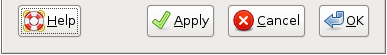
\includegraphics[height=15mm]{images/widget-keyboard-focus.png}
\caption{Billentyűzet fókusz jelzése a \textit{widget}en}
\end{center}
\end{figure}

\index{GtkWidget@\texttt{GtkWidget}!tulajdonságok!can-focus@\texttt{can-focus}}
\index{GtkWidget@\texttt{GtkWidget}!függvények!grab\_focus@\texttt{grab\_focus}}
Az egyes \textit{widget}ekre külön-külön engedhető, vagy tiltható, hogy fókuszba kerülhessenek, a \textit{can-focus} tulajdonság állításával. Az egyes \textit{widget}típusok esetében az alapértelmezés szerinti érték rendszrint megfelel a céljainknak\footnote{Ez az érték egy \texttt{GtkEntry} esetén igaz, míg egy \textit{Gtkabel} esetén hamis alapértelmezés szerint.}. Ha kódból szeretnénk átmozgatni a fókuszt az egyik \textit{widget}ről a másikra, vagy csak azt kívánjuk elérni, hogy az ablak megjelenítésekor legyen olyan \textit{widget} ami fókuszban van, akkor a \texttt{grab\_focus} függvényt kell alkalmaznunk, aminek előfeltétele a \textit{can-focus} tulajdonság igaz értéke, azaz fókuszálhatónak kell lennie, ami viszont bizonyos \textit{widget}ek (pl.: \texttt{GtkFrame}) esetén nem lehetséges.

\subsubsection{Alapértelmezett \textit{widget}}

\index{GtkDialog@\texttt{GtkDialog}
\index{gomb!jóváhagyó}
\index{gomb!ok}
\index{GtkWidget@\texttt{GtkWidget}!tulajdonságok!has-default@\texttt{has-default}}
A \texttt{GtkWindow} estén -- amit rendszerint olyan ablakhoz használunk aminek nincsenek gombjai -- ritkábban, míg \texttt{GtkDialog}} esetén csaknem mindig használt tulajdonság az alapértelmezett \textit{widget}. Ez ellentétben a fókusszal, ami inkább egy logikai tulajdonság, a felületre nincs, csak a működésre van hatással. Egy ablakon belül -- nevéből is következően -- legfeljebb egy olyan \textit{widget} lehet, mely rendelkezik ezzel a tulajdonsággal, ez rendszerint a dialógus jóváhagyó (\textit{affirmative}) gombja, jellemzően az \textit{Ok} gomb. 

\begin{figure}[H]
\begin{center}
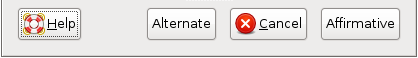
\includegraphics[height=15mm]{images/button-affirmative.png}
\caption{Gombok szokások sorrendje egy dialógusban}
\end{center}
\end{figure}

\index{billentyű!tab}
\index{billentyű!enter}
\index{GtkEntry@\texttt{GtkEntry}}
\index{GtkTextView@\texttt{GtkTextView}}
\index{GtkWidget@\texttt{GtkWidget}!tulajdonságok!can-default@\texttt{can-default}}
\index{GtkWidget@\texttt{GtkWidget}!tulajdonságok!has-default@\texttt{has-default}}
\index{GtkEntry@\texttt{GtkEntry}!tulajdonságok!activates-default@\texttt{activates-default}}
Hatása abban áll, hogy az alapértelmezett \textit{widget} -- vagyis ami esetén a \texttt{has-default} tulajdonság értéke igaz -- aktiválódik akkor, ha egy egysoros beviteli mező van fókuszban (\texttt{GtkEntry}) és akkor \textit{Enter}t nyomunk, ez is csak akkor, ha az \texttt{GtkEntry} \texttt{activates-default} tulajdonsága szintén igaz értékű. Többsoros beviteli mező (\texttt{GtkTextView}) esetén ez nem működőképes, hiszen ott az \textit{Enter} lenyomása soremelést jelent. Az alapértelmezett \textit{widget}nek a billentyűzetről való használat kényelmesebbé tételében van szerepe, hiszen ha minden szükséges mezőt kitöltöttünk egy dialógusban, akkor nem kell a megfelelő gombig -- egérrel, vagy \textit{Tab} billentyű(k) lenyomásával -- elnavigálnunk, csak egyszerűen az \textit{Enter} leütésére aktiválódik az alapértelmezett \textit{widget}.

Ahhoz, hogy egy \textit{widget} egyáltalán számításba kerüljön, mint potenciális alapértelmezett \textit{widget}, ahhoz először a \texttt{can-default} tulajdonságának kell igaznak lenni, ilyen \textit{widget} több is lehet egy ablakon belül, melyek közül aktuálisan alapértelmezetté \texttt{GtkWidget} osztály \texttt{garb\_default} függvényével tehetünk egyet, így annak \texttt{has-default} értékkel igazzá válik, míg az ablak korábbi alapértelmezett \textit{widget}e, már ha volt ilyen, esetén a tulajdonság értéke természetesen hamis lesz.

\subsection{Vezérlő elemek}
\label{sec:windowvsdialog}

Amennyiben a szükséges tartalmi elemeket elhelyeztük az ablakban, a vezérlő elemekkel is hasonlóan kell eljárnunk. A különböző célokra használt ablakok különböző vezérlő elemeket kívánnak meg, amik az egyes típusokként erős hasonlóságot mutatnak. Egy főablak csak kivételes esetekben tartalmaz az eddigiekben tárgyalt gombokat, a vezérlés általában menükkel, a \textit{toolbar}on elhelyezett gombokkal történik (\ref{fig:windowprimary} ábra).

\includetwingraphics
{Főablak}
{window-primary.png}
{windowprimary}
{Dialógus}
{window-dialog.png}
{windowdialog}
{Tipikus ablakszerkezetek\cite{gnomehig}}
{windowtypes}

A főablakból nyíló különböző célú ablakok, melyek például egy adott elem tulajdonságainak beállítására, egy bonyolultabb funkció lépésenként történő megvalósítására, az alkalmazás egészének konfigurálására, egy folyamat nyomkövetésére, esetleg a felhasználó informálására, figyelmeztetésére szolgálnak, közvetlenül, vagy közvetve a \texttt{GtkDialog} típusból szármáznak, saját gombsorral látjuk el őket. Tipikus példa erre egy elem tulajdonságainak szerkesztésére használt dialógus (\ref{fig:windowdialog} ábra).

\subsubsection{\texttt{GtkDialog}}
\label{sec:dialogbuttonadd}
\index{GtkDialog@\texttt{GtkDialog}}

A \textit{C}, illetve a \textit{Python} nyelvű változat mutat némi különbözőséget a \textit{C++} változathoz képest a gombok hozzáadásának mikéntjében. Előbbiek esetén ugyanis több gombot is hozzáadhatunk egyszerre a dialógoshoz, egymás után sorolva a \texttt{button\_text} és a \texttt{response\_id} paramétereket. A paraméterlistát a \textit{C} változat esetén \texttt{NULL} értékkel kell zárnunk, különben változatos programhibákkal fogunk szembesülni, erre a \textit{Python} esetén nincs szükség, mivel itt a hívott fél tisztában van az átadott paraméterek számával.

\lsttriplesource
[numbers=none]
{sources/dialog_button_add.h}
{sources/dialog_button_add.hpp}
{sources/dialog_button_add_init.py}
{Gombok hozzáadása \texttt{GtkDialog}hoz}
{lst:dialogbuttonaddh}

\index{GtkStockId@\texttt{GtkStockId}}
A választott nyelvi változattól függetlenül igaz, hogy a \texttt{button\_text} paramétere vagy az általunk vágyott felirat szövege lehet, vagy egy \textit{stock ID} (\textit{Ok} gomb esetén például \texttt{GTK\_STOCK\_OK}).

\begin{figure}[H]
\begin{center}
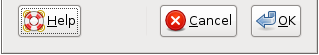
\includegraphics[height=13mm]{images/button-alternate.png}
\caption{Egy tipikus gombsor}
\end{center}
\end{figure}

Egy fenti elrendezésű -- amúgy meglehetősen szokványos -- gombsor az alábbi kódrészletekkel hozható létre az egyes nyelvek esetén. Az eltérés nem számottevő, nem tartalmaz semmilyen olyan különbözőséget, ami a korábbiakban már ne került volna ismertetésre.

\lsttriplesource
[numbers=none]
{sources/dialog_button_add.c}
{sources/dialog_button_add.cc}
{sources/dialog_button_add.py}
{Tipikus gombsor hozzáadása \texttt{GtkDialog}hoz}
{lst:dialogbuttonadd}

\subsubsection{\texttt{GtkMessageDialog}}
\label{sec:messagedialog}
\index{GtkMessageDialog@\texttt{GtkMessageDialog}}

Létezik a \texttt{GtkDialog} típusnak egy -- a gombok hozzáadása szempontjából érdekes sajátossággal bíró -- specializált változata, melyet a felhasználóval történő kommunikáció céljaira használunk, s mely ennek megfelelően rendszerint csak az üzenet szövegét, illetve a válasz megadásához szükséges vezérlő elemeket tartalmazza.

\includetwingraphics
{Információs üzenetablak}
{message-dialog-information.png}
{messagedialoginformation}
{Hiba üzenetablak}
{message-dialog-error.png}
{messagedialogerror}
{Tipikus üzenetablakok}
{messagedialogtypes}

Az ábrákon látható dialógusokat -- a szövegezéstől eltekintve -- csak típusuk különbözteti meg egymástól. A bal oldali (\ref{fig:messagedialoginformation}) egy információs ablak, míg a jobb oldali (\ref{fig:messagedialogerror}) egy hibadialógus. Az egyik szembeötlő különbség az ablakok között az ikon, amit az üzenetablak típusa határoz meg. A fenti két típuson kívül még két saját ikonnal rendelkező típus (\textit{question} és \textit{warning}) létezik, illetve készíthetünk ikon nélküli változatot, aminél módunk van saját ikon megadására.

Az üzenetablak típus eltérése, vagy inkább specialitása a \texttt{GtkDialog} típushoz képest nem csak a típus megadásának lehetőségére korlátozódik. A kifejezetten a szoftver és a felhasználó közötti ``üzenetváltás'' célját szolgáló \textit{widget} rendelkezik beépített elemekkel az üzenet megjelenítésére. A felhasználóval közölni kívántakat egy elsődleges és egy másodlagos (\texttt{primary-text}, \texttt{secondary-text}) részre bonthatjuk, ahol az előbbi egy rövid, csak a helyzet leglényegesebb elemit tartalmazó, egy mondatos összefoglalója a közölni kívánt információnak, vagy a javasolt kívánt műveletnek, míg az utóbbi ennek mélyebb, részletekbe menő kifejtése leírása, ami tájékoztatja a felhasználót a felmerült helyzet okairól, esetleges mellékhatásairól. Az esetek többségében a felhasználónak már az elsődleges szöveg elolvasását követően meg kell tudni hoznia döntését, a másodlagos szöveg a döntés alátámasztására, az esetleges kétségek eloszlatására szolgál.

A harmadik specialitás -- a gombok felhelyezésének mikéntje -- a vezérlő elemek szempontjából is említésre méltó. Azzal együtt, hogy \textit{dialog} típusnál ismertetett módszer az öröklődés okán természetesen itt is használható, mivel azonban a leggyakrabban használt gombkombinációk száma erősen korlátos, így ezek közül létrehozáskor választhatunk. Lehetséges értékek eredményeként vagy egyedüliként a \textit{Bezárás}, \textit{Ok}, \textit{Mégse} gombok, vagy a \textit{Ok}/\textit{Cancel}, \textit{Igen}/\textit{Nem} párosok kerülnek a dialógusra.

\lsttriplesource
[numbers=none]
{sources/message_dialog_create.h}
{sources/message_dialog_create.hpp}
{sources/message_dialog_create.py}
{\textit{MessageDialog} létrehozása}
{lst:messagedialogcreate}

 \index{GLib@\texttt{GLib}!makrók!G\_GNUC\_PRINTF@\texttt{G\_GNUC\_PRINTF}}
A \textit{C}, illetve a \textit{Python} nyelvű változatok, ellentétben a \textit{C++}-os megvalósítással nem egyetlen paraméterként várják az üzenetablak elsődleges szövegét, hanem egy \texttt{printf}-stílusú formátumleírót és az annak megfelelő paramétereket vesznek át. Ennek típusbiztosságáról a \textit{C} változat esetén a \texttt{G\_GNUC\_PRINTF} makró gondoskodik, már amennyiben a \textit{GNU C} fordítót használjuk. Ebben az esetben fordítási idejű figyelmeztetést kapunk ha paramétereink nem felelnek meg a formátumleíróban megadottaknak.

\subsection{Megjelenítés}

Több lehetőség kínálkozik, ha egy ablakot, illetve annak tartalmát szeretnénk megjeleníteni. Használhatjuk egyrészről, a \texttt{GtkWidget}, a \texttt{GtkWindow}, illetve a \texttt{GtkDialog} típus által adott módszereket.

\subsubsection{\texttt{GtkWidget}}

\index{GtkWidget@\texttt{GtkWidget}!függvények!show@\texttt{show}}
\index{GtkWidget@\texttt{GtkWidget}!függvények!show\_all@\texttt{show\_all}}
A korábban már tárgyalt \texttt{show} függvényt, ami megjeleníti a \textit{window}t, de csak a \textit{window}t, annak gyerekeit nem. Lévén a \textit{window} egy konténer típus, helyezhetünk el további \textit{widget}eket benne, amiknek a megjelenítéséről vagy már korábban gondoskodnunk kell -- mondjuk egy \texttt{show} hívással --, vagy megtehetjük a szülő és az összes gyerek megjelenítését egyszerre a \texttt{show\_all} függvénnyel.

\subsubsection{\texttt{GtkWindow}}

\index{GtkWindow@\texttt{GtkWindow}!függvények!present@\texttt{present}}
Egy ablak esetén nem csupán a puszta megjelenítés lehet szempont, hanem az is, hogy a felhasználó az ablakot észre is vegye. Ez az estek túlnyomó többségében adott, hiszen valamilyen felhasználói interakció révén jelenik meg az új ablak. Ha viszont nem erről van szó akkor szükséges lehet az megjelenítésen túl más ablakok általi takarás megszüntetésére, a tálcáról való felhozatalra, az aktuális desktopra  történő mozgatásra, a fókusz (\ref{sec:widgetfocus}) átadására, mely műveletek mind függhetnek mind a platformtól, mind az ablakkezelőtől, mind pedig a felhasználói beállításoktól. Erre használható a \texttt{present} függvény. Kezeljük azonban kellő óvatossággal ezt a függvényt, hiszen mindannyian bosszankodtunk már egy kellő indok nélkül, váratlanul megjelenő ablak miatt.

\subsubsection{\texttt{GtkDialog}}

\index{main loop}
\index{GtkDialog@\texttt{GtkDialog}!függvények!run@\texttt{run}}
\index{GtkWindow@\texttt{GtkWindow}!tulajdonságok!modal@\texttt{modal}}
Egy \textit{window} típusú ablak esetén -- mivel jellemzően nincsenek az ablakon gombok és nem modálisak -- nincs igazán szükségünk arra, hogy -- a kód futásának szempontjából helyben -- kivárjuk a felhasználó reakciót. A \textit{dialog} típus ezzel szemben általában egy felhasználói interakció révén jelenik meg (pl.: egy elem tulajdonságait, vagy az applikáció beállításait szerkesztő ablak) és jelentős részben valamilyen döntés elé állítja a felhasználót (különösen igaz ez az üzenet ablakoknál, ahol kérést teszünk fel), melynek eredményéről szeretnénk értesülni. A \texttt{GtkDialog} típus \texttt{run} függvénye -- ahogy azt a következőekben (\ref{sec:dialogresponse}) részletesen is tárgyaljuk -- pontosan ezt a célt szolgálja. Egyrészről várakozik a felhasználó interakció -- amihez természetesen szükséges a \textit{main loop} futtatása -- majd visszatérési értékként az ablak ``futtatásának'' eredményét, vagyis a kiválasztott vezérlő elem -- az ablak elkészítésekor megadott -- \textit{response id}-t adja vissza. Mint látható, a függvény nem kifejezetten a dialógus megjelenítését szolgálja, az hasznos mellékhatásként mégis megtörténik.

\subsection{Bezárás}

A \textit{window} tehát leginkább a bezárás kapcsán állít kihívást elénk, melyet függően attól, mit szeretnénk elérni annak hatására, hogy a felhasználó az ablak bezárását kezdeményezte, több lehetséges megoldás, az egyes megoldásokra, pedig több módszer is kínálkozik.

\subsubsection{Blokkolás}

Kezdjük a legegyszerűbbnek látszó esettel, vagyis azzal, hogy semmilyen hatása ne legyen annak ha felhasználó az ablak bezárását kezdeményezi. Nyilván megfontolandó, hogy ezt tegyük, hiszen a felhasználó sem véletlenül akarja, amit akar, de ha mondjuk azt szeretnénk kikényszeríteni, hogy a főablakunkból csak a Fájl menüpont ``Kilépés'' almenüpontjára kattintva lehessen bezárni, akkor ez egy lehetséges megoldás\footnote{Ne becsüljük azonban alá se a felhasználói találékonyságot, se a felhasználói környezetek változatosságát. Semmiképp ne hagyatkozzunk arra, hogy egy adott módszer a felhasználó számára véleményünk szerint nem érhető el.}.

A feladat megoldása a korábban már tárgyalt \textit{delete-event} szignál kezelésében rejlik. Ahogy arról szó esett ez a szignál váltódik minden ablakon (\textit{toplevel window}), illetve minden az ablakban lévő \textit{widget}en, mikor a felhasználó az ablak bezárását kezdeményezi. A szignál két külön említésre is méltó sajátossággal is rendelkezik:

\begin{enumerate}
 \item A szignált kezelni kívánó függvénynek egy \textit{bool} értékkel kell visszatérnie, ami azt jelzi a \textit{GTK} felé, hogy az adott függvény kezelte-e az eseményt, egyszersmind nincs szükség a további kezelő függvény meghívására. A \textit{GTK} következésképp addig hívja sorra az szignálra ``feliratkozott'' függvényeket (\textit{signal handler}) -- köztük ha van ilyen, akkor az alapértelmezett szignálkezelő függvényt (\textit{default signal handler}) amíg egyikük \textit{true} értékkel nem tér vissza.
 \item Ha minden ilyen függvény \textit{false} értékkel tér vissza, azaz a szignál további propagálását kéri a \textit{GTK}-tól, akkor konkrétan a \texttt{delete-event} esetében a \textit{GDK} alapértelmezett eseménykezelője (\textit{default event handler}) fut le, ami meghívja az ablak destruktorát.
\end{enumerate}

Fentiek alapján ahhoz, hogy megelőzzük az ablak bezárását -- vagyis hogy ne történjen semmi -- el kell érnünk, hogy az alapértelmezett eseménykezelő ne hívódjon meg, azaz az általunk felkötött szignálkezelő \textit{true} értékkel kell hogy visszatérjen, jelezve azt, hogy az eseményt kezeltük, a további szignálkezelő függvények meghívására nincs szükség. Ebben az esetben ez azt is jelenti, hogy az alapértelmezett eseménykezelő sem hívódik meg. Ehhez definiálnunk kell a szignálkezelő  függvényeket, ami a korábbi (\lstref{lst:windowminimal}\footnote{A sorszámozás az eredeti példába való beillesztés pontját mutatja.}) példát kiegészítve az alábbihoz hasonló módon tehetünk meg,

\lsttriplesource
[firstnumber=2]
{sources/window_persistent_callback.c}
{sources/window_persistent_callback.cc}
{sources/window_persistent_callback.py}
{Szignálkezelő függvény perzisztens ablakhoz}
{lst:windowpersistentcallback}

majd ezeket a függvényeket a \texttt{delete-event} szignálra be is kell kötnünk\footnote{A sorszámozás az eredeti példába való beillesztés pontját mutatja.}.

\lsttriplesource
[firstnumber=12]
{sources/window_persistent_connect.c}
{sources/window_persistent_connect.cc}
{sources/window_persistent_connect.py}
{Szignálkezelő függvény bekötése perzisztens ablakhoz}
{lst:windowpersistentconnect}

Ha az adott szignál alapértelmezett szignálkezelő függvénnyel is rendelkezik -- ami a \textit{widget} osztály-leírójában kerül megadásra -- és magunk akarjuk a szignált kezelni, akkor szükségessé válik, hogy a saját kezelő függvényünk még az alapértelmezett előtt hívódjék meg, ami további praktikák bevetését igényli, amiről egy másik részben esett részletesebben szó.

\index{Gtk@\texttt{Gtk}!függvények!true@\texttt{true}}
\index{Gtk@\texttt{Gtk}!függvények!false@\texttt{false}}
Ha a saját szignálkezelő függvény írását kissé túlzónak találjuk egy olyan egyszerű feladat ellátására, mint egy \textit{true} értékkel való visszatérés, akkor nem tévedünk, sőt a \textit{GTK+} fejlesztői is gondoltak erre és megalkották a \texttt{gtk\_true}, illetve a \texttt{gtk\_false} nevű függvényeket, melyek semmi egyebet nem tesznek, mint a nevüknek megfelelő értékkel térnek vissza, így a fenti példa szignálkezelő függvényei elhagyhatók, hiszen azok \textit{GTK+} által adott -- ekvivalens funkciójú -- függvényekkel helyettesíthetőek.

\lstinputsource
[language=C]
{sources/window_persistent_simple.c}
{Egyszerűsített szignálkezelő függvény bekötése}
{lst:windowpersistentsimple}

\subsubsection{Eltüntetés}

Folytassuk másodikként azzal az eshetőséggel, ha el szeretnénk tüntetni az ablakot, aminek a bezárását a felhasználó kezdeményezte. Az előző szituációhoz hasonlóan most is több módszer adódik a feladat megoldására.

\index{GtkWidget@\texttt{GtkWidget}!függvények!hide@\texttt{hide}}
\index{GtkWidget@\texttt{GtkWidget}!szignálok!delete-event@\texttt{delete-event}}
A fent tárgyalt perzisztens ablakot eredményező szignálkezelők (\lstref{lst:windowpersistentcallback}) ismeretében a legnyilvánvalóbb megoldás, hogy még mielőtt visszatérnénk az adott függvényekből a \texttt{hide} függvény segítségével eltüntetjük az adott ablakot. A megoldás jó és működőképes megoldás lehet, ugyanakkor számolnunk kell azzal, hogy az ablak csak eltűnik, de nem feltétlenül semmisül meg. A már korábban is használt minimális példa azon kiegészítését is figyelembe vesszük, ahol a \texttt{delete-event} szignálra a \textit{main loop} futását megszakító függvényt hívjuk, akkor azt fogjuk tapasztalni, hogy az ablakunk eltűnik ugyan, de a mögöttes működés már nagyban attól függ a két implementációt (\lstref{lst:windowpersistentcallback}) miként vontuk össze. Ha a saját szignálkezelő függvényünket kötjük be előbb a \texttt{delete-event} szignálra, akkor az -- a visszatérési értéke révén -- leállítja a szignál további kezelését, vagyis a szignálkezelő függvények sorának meghívását is, így az ablak a saját kezelő függvényünk (\texttt{on\_delete\_event}), a \texttt{hide} hívással kiegészítve eltünteti az ablakot, de a következő szignálkezelő -- ami kiléptetné a \textit{main loop}ot -- már nem hívódik meg. Ha a felkötés sorrendje fordított, akkor előbb kilép a \textit{main loop} és csak ezután hívódik meg saját függvényünk, ami egyrészről elrejti az ablakot, másrészről blokkolja a további kezelést, aminek végső soron nem lehet hatása, hiszen a \textit{main loop} már kilépett.

Amennyiben a célunk csupán az ablak eltüntetése egyszerűbben is elérhetjük ugyanezt, hiszen a \texttt{hide} függvény közvetlenül -- pontosabban egy beépített \textit{GTK+} keresztül -- is beköthető a \texttt{delete-event} szignálra. Ezt kényelmi funkciót a \textit{gtkmm} esetén elveszítjük -- hasonlóan az előző példához --, mivel az általunk használni kívánt szignálkezelő függvény deklarációja nem egyezik meg az előírttal, így tehát ezt a ``kényelmet'' a típusbiztosság oltárán fel kell áldozni.

\lstinputsource
[language=C]
{sources/window_hide_on_delete_event_simple.c}
{Egyszerűsített szignálkezelő függvény bekötése}
{lst:windowpersistentsimple}

Ha nem ragadunk le a könnyen érthető, ám nem túl életszerű minimális példánknál, akkor az mondható el, hogy ablakokat -- legyenek azok \texttt{GtkWindow}, vagy \texttt{GtkDialog} típusúak --, valamilyen felhasználói interakcióra reagálva hozunk fel, valamilyen kezelő függvényben. Az bezáráskori elrejtés akkor lehet hasznos számunkra, ha nem akarjuk újra és újra elkészíteni az ablakot az adott felhasználói műveletre. Erre lehet példa mondjuk egy névjegy (\textit{about}) ablak, aminek a tartalma nem változik a program futása során, így azt az alkalmazás indulásakor, vagy az első megtekintéskor létrehozzuk, utána már elegendő csak elrejteni, vagy újra megjeleníteni. Másik példa lehet egy státusz jellegű információkat megjelenítő ablak, amiben úgymond gyűjteni tudjuk az adatokat és ha a felhasználó be is zárja az ablakot, mi az elrejtés után az adatgyűjtést és az ablak tartalmának frissítését tovább fojtatjuk, majd az újbóli megjelenítéskor már a naprakész információk jelennek meg.

\subsubsection{Megszüntetés}

\index{GtkWidget@\texttt{GtkWidget}!szignálok!delete-event@\texttt{delete-event}}
Mint az a fentiekből már kiderült -- függetlenül attól, hogy \texttt{GtkWindow}, \texttt{GtkDialog}, vagy ezekből származó típusokról van-e szó --, a \textit{delete-event} szignál kiváltódását -- ha egyebet nem teszünk -- az ablak destruktorának meghívás fogja automatikusan követni, ami az esetek túlnyomó többségében meg is felel a céljainknak.

\subsection{Eseménykezelés}
\label{sec:dialogresponse}

\subsubsection{Szinkron}

A \texttt{GtkDialog} és a \texttt{GtkWindow} típusok közötti eltérések (\ref{sec:windowvsdialog}) közül a legszámottevőbb -- mivel ehhez tartozik a legtöbb beépített szolgáltatás --, a vezérlő elemek, azaz a gombok kezelése. A \texttt{GtkDialog} nem csupán arra ad lehetőséget, hogy a gombokat egy erre a célra készült konténerbe helyezzük el -- ezt magunk is megtehetnénk minden különösebb erőfeszítés nélkül --, hanem az ezeken végzett felhasználói interakciókat is egyszerűen nyomon követhetjük. Választhatunk az adott (kód)környezetben számunkra kényelmesebb -- szinkron, illetve aszinkron eseménykezelés közül. Előbbi esetén helyben\footnote{Az ablak létrehozásának helyén.} tudjuk kezelni az eseményeket, utóbbi viszont eseménykezelő függvények megírását és bekötését teszi szükségessé.

\lsttriplesource
{sources/dialog_minimal.c}
{sources/dialog_minimal.cc}
{sources/dialog_minimal.py}
{Minimál példa \texttt{GtkDialog}hoz}
{lst:dialogminimal}

\index{main loop}
\index{GtkDialog@\texttt{GtkDialog}!függvények!run@\texttt{run}}
\index{GtkDialog@\texttt{GtkDialog}!szignálok!response@\texttt{response}}
\index{GtkWidget@\texttt{GtkWidget}!szignálok!unmap@\texttt{unmap}}
\index{GtkWidget@\texttt{GtkWidget}!szignálok!destroy@\texttt{destroy}}
\index{GtkWidget@\texttt{GtkWidget}!szignálok!delete-event@\texttt{delete-event}}
A \texttt{run} függvény (\ref{dialogminimalc:dialogrun}.) egyrészről függvényeket köt be a szükséges szignálokra (\texttt{response}, \texttt{unmap}, \texttt{delete-event}, \texttt{destroy}), majd egy saját \textit{main loop}ot futtatásán belül kezeli az említett eseményeket. Ha ezek közül bármelyik bekövetkezik, akkor a \textit{main loop} futása megszakad, és a \texttt{run} függvény a megfelelő értékkel visszatér. Ennek kezelése tipikusan egy \texttt{if}, vagy egy \texttt{switch} szerkezeten belül történik.

Ha a fenti minimális példát a korábbi, gombok hozzáadását tartalmazó forrással (\lstref{lst:dialogbuttonadd}) egészítjük ki\footnote{A változók deklarációinak hozzáadása szükséges a fordíthatóság érdekében.}, mondjuk az alábbihoz hasonló módon kezelhetjük a felhasználói döntés eredményeként kapott választ (\texttt{response}).

\lsttriplesource
[firstnumber=12]
{sources/dialog_run.c}
{sources/dialog_run.cc}
{sources/dialog_run.py}
{Minimál példa \texttt{GtkDialog}hoz}
{lst:dialogrun}

\index{Gtk@\texttt{Gtk}!konstansok!RESPONSE\_DELETE\_EVENT@\texttt{RESPONSE\_DELETE\_EVENT}}
Itt az egyszerűség kedvéért csak az \textit{Ok}, illetve a többi gomb kerültek megkülönböztetésre, így ha a \textit{Mégse}, illetve a \textit{Súgó} gomb aktiválódott, akkor is a \texttt{switch} szerkezet \texttt{default} ága (\ref{dialogrunc:switchcasedefault}) fut le. Kérdés azonban, hogy ha az imént megismert \texttt{delete-event} szignál váltódik ki az ablak bezáródásának hatására, annak mi lesz az eredménye. A válasz egyszerű, hiszen a \texttt{switch} első ágára (\ref{dialogrunc:switchcaseok}) nem futhatunk rá, tehát marad itt is a \texttt{default} ág. Ha külön szeretnénk kezelni ezt az esetet, akkor a \texttt{RESPONSE\_DELETE\_EVENT} konstans kezelésére kell egy új ágat beillesztenünk.

\index{GtkDialog@\texttt{GtkDialog}!függvények!run@\texttt{run}}
\index{Gtk@\texttt{Gtk}!konstansok!RESPONSE\_NONE@\texttt{RESPONSE\_NONE}}
Nem minden esetet fedtünk azonban le, elképzelhető ugyanis, hogy a dialóg felszabadul, míg a \texttt{run} függvény fut. Ebben az esetben a visszatérési érték \texttt{RESPONSE\_NONE} lesz, így ezt az esetet is meg lehet különböztetni a többitől, azonban mégsem tanácsos. Helyette, ha mindenképpen meg akarjuk szakítani a \texttt{run} futását, akkor a \texttt{resposne} függvényt hívhatjuk, aminek eredményeként a \texttt{run} a \texttt{resposne}-nak paraméterként átadott értékkel tér vissza.

\index{GtkWidget@\texttt{GtkWidget}!függvények!show@\texttt{show}}
Az élelmesebbek megfigyelhetik, hogy \textit{dialog} példaprogramból (\lstref{lst:dialogminimal}) a \textit{window} hasonló példájához (\lstref{lst:windowminimal}) kimaradt a \texttt{show} függvény hívása, ami annak tudható be, hogy a \texttt{run} ezt megteszi helyettünk, ahogy a dialógusunkat is modálissá teszi a \texttt{run} futásának idejére.

\subsubsection{Aszinkron}

\index{GtkDialog@\texttt{GtkDialog}!szignálok!response@\texttt{response}}
Ha valamilyen oknál fogva lemondanák a \texttt{run} adta kényelemről, lehetőségünk van az aszinkron kezelésre. Ebben az esetben a \texttt{run} helyett a \textit{show} függvényt hívjuk, illetve egy saját függvényt -- melyben elvégezzük a számunkra szükséges műveleteket -- kötünk be a \texttt{response} szignálra. Ezt a módszert használva ebben a függvényben kell gondoskodnunk az ablak felszabadításáról is, már amennyiben nem csak a \texttt{delete-event} esemény hatására szeretnénk, hogy ez megtörténjen. A \texttt{response} szignál paraméterei között a \texttt{response\_id} is szerepel, így a függvény tartalma hasonló lehet a \texttt{run} hívást követő kódhoz (\lstref{lst:dialogrun}). Működésben azonban van némi különbség, hiszen a \texttt{delete-event} alapértelmezett működésének megváltoztatására például nincs mód.

Az aszinkron a megoldásra lehet egy másik példa, ha a lehetséges választások mindegyike ugyanazzal az eredménnyel kell járjon, például be kell záródjon az ablak. Ennek olyan leginkább helyzetekben van realitása, ahol csupán egy (pl.: \textit{Bezárás}) gomb jelenik meg az ablakon. Erre lehet példa egy olyan üzenetablak (\textit{MessageDialog}), amiben nem egy kérdést teszünk fel, hanem csupán informáljuk a felhasználót.

\lstinputsource
[language=C]
{sources/dialog_destroy_on_response_simple.c}
{Egyszerűsített \textit{response}-kezelő függvény bekötése}
{lst:windowpersistentsimple}

\subsection{Saját eseménykezelő}

Ha a fentiekben vázoltak valamilyen oknál fogva nem elégítenék ki igényeinket, vagy már egyébként is alkalmasabb módszernek látszik egy saját \textit{widget} implementálása akkor nem kell egyebet tennünk, minthogy az ősosztály eseménykezelő függvényét felüldefiniáljuk a nyelvi változatnak megfelelő módon.

\lsttriplesource
{sources/mywindow_part.c}
{sources/mywindow_part.cc}
{sources/mywindow_part.py}
{Eseménykezelő felüldefiniálása saját \textit{widget}osztályban}
{lst:mywindowpart}

Az objektum-orientált megvalósítások esetén ez egy lényegesen kisebb erőfeszítést igénylő feladat. Ahogy ezt a fenti kódrészlet is mutatja a \textit{C} változatból épp csak a leglényesebb rész emelhető ki egy jó tucatnyi sorban\footnote{A teljes \textit{C} kód egy \ref{mywindowc:lastline} soros \texttt{.c}, illetve egy \ref{mywindowh:lastline} soros \texttt{.h} állományból áll.}, addig a csaknem teljes értékű \textit{C++}, \textit{Python} kódok ennek a felét sem teszi ki.

\section{Platformfüggő sajátosságok}

Bár a \textit{GTK} -- a \textit{GDK}\footnote{GIMP Drawing Kit}, illetve a \textit{Glib} függvénykönyvtárakon keresztül -- komoly platformfüggetlenséget biztosít, mégis számolnunk kell a különbségekkel, különösen az ablakok kezelése kapcsán. Ezek közül itt csak a két legfontosabbat emeljük ki.

\subsection{Ablakkezelő}

Bizonyos értelemben maga a az ablakkezelő is egy platform, hisz ahogy az operációs rendszerek a tőlük elvárt funkciókat -- mint amilyen például a fájlkezelés -- a maguk módján valósítják meg, úgy az ablakkezelő rendszerek is saját szisztémájuk szerint teszik ezt. Bizonyos funkciók csak néhány ablakkezelő implementál, addig másokat csaknem minden ilyen rendszer megvalósít, bár arra nem számíthatunk, hogy az egyes megvalósítások minden részletben megegyeznek.

Az ablakkezelők különbözőségei fejlesztési oldalról azzal a következménnyel járnak, hogy még akkor is szembe kell néznünk a platformok sajátosságai által okozott nehézségekkel, ha egyébként alkalmazásunkat nem használjuk több különböző\footnote{Ebben a tekintetben a \textit{Linux} alapú rendszereket közel azonosnak tekinthetjük} operációs rendszer alatt.

\index{GtkWindow@\texttt{GtkWindow}!függvények!stick@\texttt{stick}}
\index{GtkWindow@\texttt{GtkWindow}!függvények!iconify@\texttt{iconify}}
\index{GtkWindow@\texttt{GtkWindow}!függvények!maximize@\texttt{maximize}}
\index{GtkWindow@\texttt{GtkWindow}!függvények!fullscreen@\texttt{fullscreen}}
\index{GtkWindow@\texttt{GtkWindow}!függvények!set\_keep\_above@\texttt{set\_keep\_above}}
Még az olyan egyszerű és széles körben megvalósított funkciók kapcsán, mint amilyen maximalizálás, vagy a minimalizálás (\texttt{maximize}, \texttt{iconify}) kételkednünk kell a mögöttes implementáció meglétében, illetve figyelembe kell vennünk az egyes megvalósítások különbözőségeit, vagyis nem alapozhatunk ezen függvények meghívását követően arra, hogy az ablak abba az állapotba kerül, amire számítottunk. Akár az előbbiek említett funkciókra, akár mondjuk az ablak előtérben tartására (\texttt{keep\_above}), akár teljes képernyőméretre nagyításra (\texttt{fullscreen}), akár az összes munkaterület (\textit{desktop}) való egyszerre történő meg megjelenítésre (\texttt{stick}) kérjük az ablakkezelőt, nem bizonyos, hogy kérésünk teljesül. Ennek csak az egyik oka az, hogy az ablakkezelő nem támogatja az adott funkciót, a másik pedig, hogy kérésünket követően valaki más az előző, vagy éppen mindkettőtől eltérő állapot állít be. Ennél fogva ügyelnünk kell arra, hogy egy ilyen helyzetre programunk fel legyen készülve.

\index{GtkWindow@\texttt{GtkWindow}!függvények!set\_deletable@\texttt{set\_deletable}}
\index{GtkWindow@\texttt{GtkWindow}!függvények!set\_skip\_taskbar\_hint@\texttt{set\_skip\_taskbar\_hint}}
Az ablak dekorációja a másik olyan terület, ahol kéréseket (\textit{hint}) intézhetünk az ablakkezelő felé. Hasonlóan azonban a fent tárgyaltakhoz itt is igaz, hogy célszerű ellenőrizni feltételezéseinket arra vonatkozólag, hogy kérésünk úgy és abban a formában hajtódik végre, ahogy azt mi elgondoltuk. Számos olyan eset lehetséges az ablak dekorációján található bezáró gomb megjelenítésének tiltásától (\texttt{deletable}), az ablak \textit{taskbar}ból történő kihagyásáig (\texttt{skip\_taskbar\_hint}) melynek implementációs részletei teljes egészében az ablakkezelőtől függenek.

\subsection{Vezérlő elemek}

\index{gomb!menekülő}
\index{gomb!jóváhagyó}
\index{GtkDialog@\texttt{GtkDialog}!függvények!set\_alternative\_button\_order@\texttt{set\_alternative\_button\_order}}
\index{GtkDialog@\texttt{GtkDialog}!függvények!set\_alternative\_button\_order\_from\_array@\texttt{set\_alternative\_button\_order\_from\_array}}
A \textit{GTK} alapértelmezés szerint a gombokat a \textit{GNOME Human Interface Guideline}\cite{gnomehig} (\textit{HIG}) által javasolt elrendezését alkalmazza, vagyis a jóváhagyó (\textit{affirmative}) gomb a jobb oldalon a szélső pozícióba kerül, míg a menekülő gomb (\textit{cancel}) ettől balra kerül. Ha eltérő -- úgymond alternatív elrendezést -- szeretnénk, akkor azt a \texttt{set\_alternative\_button\_order} függvény segítségével egy korábbi példát (\lstref{lst:dialogbuttonadd}) kiegészítve az alábbi módon állíthatjuk be.

\lsttriplesource
[numbers=none]
{sources/dialog_button_order.c}
{sources/dialog_button_order.cc}
{sources/dialog_button_order.py}
{Alternatív gombsorrend beállítása}
{lst:dialogbuttonorder}

Amennyiben az üzenetablakoknál megismert (\ref{sec:messagedialog}) páros gombok (\textit{Ok}/\textit{Cancel}, \textit{Igen}/\textit{Nem}) valamelyikét használjuk, akkor ezt a sorrendállítást a \textit{GTK} megteszi helyettünk.

\section{A kód}

\subsection{Fordítás és linkelés}

A korábbiakhoz hasonlóan az alábbi parancssorok segítségével fordíthatóak programjaink.

\lstcompiles
{gtk_sourcefile.c}{gtk_binary}
{gtkmm_sourcefile.cc}{gtkmm_binary}

\subsection{Futtatás}

A futtatással ezúttal is a forrásfájlok -- egyszersmind a fordítás -- könyvtárában érdemes próbálkoznunk, a példaprogram nevétől függően a \texttt{./futtatható\_bináris} parancs kiadásával.

\subsection{Eredmény}

Bármily hihetetlen ezúttal sem történik semmi egyéb, mint a korábbiakban. Remélhetőleg azonban a különbség mégis érzékelhető annyiban, hogy legutóbb a meglepetéssel teli borzongást ablakunk váratlan felbukkanása, míg most a bennünk szikraként felvillanó megértés okozza.

\section{Tesztelés}

\subsection{Keresés}

\subsubsection{Applikáció keresése}

Fejlesztés közben -- már amennyiben a felhasználói felületet kódból és nem egy felülettervező program segítségével hozzuk létre -- az egyes \textit{widget}ek létrehozáskor módunkban áll egyúttal valamilyen változóval hivatkoznunk rájuk, így a későbbiekben nincs szükségünk arra, hogy az egyes \textit{widget}eket a felhasználói felületen belül keresgessük. Teszteléskor ugyanakkor a felületet készen kapjuk így az első feladat azon elemek megtalálása, amiken később valamilyen műveleteket szeretnénk végezni.

\lstdoublepysource[firstline=5, lastline=9, numbers=none]
{sources/dogtail_minimal_procedural.py}
{sources/dogtail_minimal_tree.py}
{Alapvető elemek keresése teszt \textit{tree}, illetve \textit{procedural} API használata mellett}
{lst:dogtailminimal}


\index{dogtail.tree@\texttt{dogtail.tree}!függvények!application@\texttt{application}}
Ahogy az a korábbi minimális tesztelési példában is látszott az első lépés a tesztelés során, hogy a kívánt applikációt megtaláljuk a sok egyéb futó alkalmazás között. Ha ezzel megvagyunk, akkor az applikáción belül kereshetjük meg annak ablakait, azokon belül pedig az egyes \textit{widget}eket. Előbbire a célra szolgál a \textit{Dogtail} \texttt{tree} moduljának \texttt{application} függvénye.

\index{dogtail.tree@\texttt{dogtail.tree}!függvények!application@\texttt{application}}
\index{dogtail.tree@\texttt{dogtail.tree}!függvények!application@\texttt{applications}}
A függvény mindössze egy paraméter vesz át, a keresett applikáció nevét. Ez a név jellemzően -- bár nem minden esetben -- megegyezik annak az applikáció indításához futtatott állomány nevével. Mint a későbbekben is csaknem mindig, a kísérletezés segít leginkább az applikáció felderítésében, a kereséshez használandó nevek meghatározásában. Ehhez egyrészről használhatjuk a korábban már említett \textit{Accerciser}t, ami voltaképpen egy grafikus felhasználói felület, ami az akadálymentesítéhez használt \textit{API} által megszerezhető információkat jeleníti meg struktúrált formában. Másrészről használhatjuk a \textit{Dogtail}t, a konkrét esetben a \texttt{Root} osztály \texttt{applications} függvényét, ami az összes -- az \textit{accessibilty} alrendszer számára látható -- applikációval tér vissza.

\index{dogtail.Config@\texttt{dogtail.Config}!tulajdonságok!searchCutoffCount@\texttt{searchCutoffCount}}
\index{dogtail.Config@\texttt{dogtail.Config}!tulajdonságok!searchBackoffDuration@\texttt{searchBackoffDuration}}
Az \texttt{application} függvény a \texttt{tree} modul \texttt{Application} osztályának egy, az applikációhoz tartozó példányával tér vissza, vagy ha az applikációt az újrapróbálkozásokat követően -- melyek számát a \texttt{Config} osztály \texttt{searchCutoffCount} tulajdonsága, míg a próbálkozások között tartandó szünet mértékét ugyanezen osztály \texttt{searchBackoffDuration} tulajdonsága határoz meg -- nem találja \texttt{SearchError} kivételt dob.

\subsubsection{Általános keresés}

\index{dogtail.Node\texttt{dogtail.Node}!függvények!findChild@\texttt{findChild}}
A \texttt{findChild} függvény első paramétere egy feltételhalmaz (\texttt{predicate}). Amennyiben a keresés során ennek a faltételhalmaznak megfelelő elemet találunk a közvetlen vagy közvetett leszármazottak között -- függően a \texttt{recursive} paraméter értékétől --, akkor a függvény az első ilyennel visszatér. Amennyiben nem talál megfelelő elemet és a \texttt{retry} paraméter értéke \texttt{True}, akkor újra próbálkozik a \texttt{config} objektumban foglalt beállításoknak megfelelően. Amennyiben a \texttt{retry} értéke \texttt{False} értelem szerűen összesen egy próbálkozás történik. Ha a \texttt{requireResult} paraméter értéke \texttt{True}, akkor \texttt{SearchError} kivételt dob, ha nem akkor egyszerűen \texttt{None} értékkel tér vissza. Megjegyzendő, hogy mindkét paraméter alapértelmezett értéke \texttt{True}, azaz a \textit{Dogtail} többször is próbálkozik és sikertelenség esetén \texttt{SearchError} kivételt dob.

\lstinputsource
[language=Python]
{sources/dogtail_predicate_generic.py}
{Node keresése \texttt{GenericPredicate}, illetve \texttt{findChild} függvény segítségével}
{lst:windowpersistentsimple}

\index{dogtail.Node\texttt{dogtail.Node}!függvények!findChild@\texttt{findChild}}
Ahogy látszik a \texttt{findChild} függvénynek átadott \texttt{GenericPredicate} objektum voltaképpen a keresési feltételeket zárja egy egységbe. Ezek a feltételek a név (\texttt{name}), a szerep neve (\texttt{roleName}) , leírás (\texttt{description}), illetve felirat (\texttt{label}). A működésről fontos megjegyezni, hogy a feltételhalmazban az utolsó feltétel (\texttt{label}) előnyt élvez a többivel szemben, vagyis amennyiben ezt feltételt megadjuk a másik három nem érvényesül. Ha viszont csak az első három paraméter használjuk azok egymással és kapcsolatba kerülnek, vagyis csak olyan elem lehet a keresés eredmény, ami minden feltételnek megfelel.

A feltételhalmazban megadott paraméterek értékeinek kísérleti úton meghatározását a már több alkalommal említett \textit{Accerciser} alkalmazás tud segíteni. Egyrészről megjeleníti az egyes applikációkat, azok ablakait, illetve a további gyerekelemeket fa hierarchiába szervezve. Másrészről az egyes -- amik mind egy-egy \texttt{Node} típusú objektumot jelentenek -- kapcsán megmutatja mik az objektum tulajdonsági, állapotai, a rajta végrehajtható akciók. Természetesen a későbbiekben az egyes \textit{widget}típusok ismertetésekor ezen értékekre mi is ki fogunk térni.

\index{GtkWidget@\texttt{GtkWidget}!függvények!get\_accessible@\texttt{get\_accessible}}
\index{AtkObject@\texttt{AtkObject}}
\index{AtkObject@\texttt{AtkObject}!függvények!set\_name@\texttt{set\_name}}
\index{dogtail.Node@\texttt{dogtail.Node}!tulajdonságok!roleName@\texttt{roleName}}
\index{dogtail.Node@\texttt{dogtail.Node}!tulajdonságok!name@\texttt{name}}
Az általános keresés szempontjából az imént említett néhány paraméter, illetve a \texttt{Node} osztály ezeknek megfelelő paraméterei érdemlegesek. A név attribútum (\texttt{name}) a \textit{widget} típusától -- amit a \texttt{role}, illetve annak szöveges formája a \texttt{roleName} reprezentál --, függően vesz fel értéket. Ablakok esetén annak címsorát, címkék esetén azok szövegét, olyan \textit{widget}ek esetén, amikhez címkét kapcsoltunk szintén a címke szövegét. A nevek felvett értékeinek részleteire, valamint a típusnevekre az egyes \textit{widget}típusok tárgyalásakor térünk. Maga a név explicit módon is beállítható a \textit{GTK}, pontosabban az \textit{ATK} révén, hiszen ez utóbbi interfészen keresztül történik az \textit{accessibilty} réteggel történő kapcsolattartás. Minden \texttt{GtkWidget} objektumhoz tartozik egy \texttt{AtkObject} objektum, amit a \texttt{get\_accessible} függvény segítségével kérhetünk. Az \texttt{AtkObject} a \texttt{set\_name} függvény révén adható olyan név, amire a \textit{Dogtail} használata során is hivatkozni tudunk.

\index{dogtail.Predicate@\texttt{dogtail.Predicate}}
\index{dogtail.Node@\texttt{dogtail.Node}!függvények!satisfies@\texttt{satisfies}}
\index{dogtail.Predicate@\texttt{dogtail.Predicate}!függvények!satisfiedByNode@\texttt{satisfiedByNode}}
A már említett \texttt{Predicate} osztálynak példányait felhasználhatjuk arra is, hogy csupán annyit tudjuk egy adott \texttt{Node} gyerekeként, ami megfelel a \textit{predicate} által megfogalmazott feltételhalmaznak. Ehhez a \texttt{Predicate} osztály \texttt{satisfiedByNode} függvényét kell hívnunk, arra azzal a \textit{Node} objektummal paraméterként, amire a vizsgálatot el szeretnénk végezni. Egy adott \texttt{Node} objektumról ugyanez a döntés a \texttt{satisfies} függvény hívásával hozható meg aminek viszont a \textit{predicate} a paramétere.

\subsubsection{Specializált keresés}

Létezik számos specializációja, leszármazottja a \texttt{Predicate} osztálynak, amik a gyakran használt keresések egyszerűsítésére szolgálnak. Ezek közül minden részben azokat vesszük sorra, amik az adott rész szempontjából érdekesek. Itt tehát az applikációk és ablakok keresésére szolgálok származtatásokat ismertetjük.

\paragraph{Applikáció}

\index{dogtail.Root\texttt{dogtail.Root}!függvények!application@\texttt{application}}
A \texttt{Root} osztály \texttt{application} függvénye az \texttt{Application} osztály a \texttt{tree} modul \texttt{Node} osztályából származik, ami gyakorlatilag minden olyan osztálynak őse, melyet egy keresés eredményeként visszakaphatunk (\texttt{Application}, \texttt{Root}, \texttt{Window}).

\lstinputsource
[language=Python]
{sources/dogtail_find_application.py}
{Applikáció keresése \texttt{application} függvénnyel, illetve \texttt{IsAnApplicationNamed} objektummal}
{lst:windowpersistentsimple}

\index{dogtail.Node\texttt{dogtail.Node}!függvények!findChild@\texttt{findChild}}
\index{dogtail.Predicate@\texttt{dogtail.Predicate}}
Ahogy látszik az \texttt{application} függvény nem más, mint egy specializáció, ami tulajdonképpen \texttt{Node} osztály \texttt{findChild} általános keresőfüggvényét hívja paraméterként egy \texttt{IsAnApplicationNamed} osztály egy objektumával, ami a \texttt{Predicate} osztályból származik és példányosításkor a keresendő applikáció nevét veszi át paraméterként.

\paragraph{Ablak}

Hasonlóan az applikáció kereséséhez az ablakok keresésére is létezik a \texttt{Predicate} osztályból származó saját osztály. Mind a \texttt{IsAWindowNamed}, mind a \texttt{IsADialogNamed} konstruálásához csak az ablak címsorát kell megadnunk. A két külön osztályra mindössze azért van szükség, mert a \texttt{GtkWindow} és a \texttt{GtkDialog} típusok a \textit{Dogtail} reprezentáció más \texttt{roleName} értékkel rendelkeznek (\texttt{frame}, \texttt{dialog}), ahogy az a egyezést vizsgáló függvénnyek implementációjából is látszik.

\lstinputsource
[language=Python]
{sources/dogtail_find_window.py}
{Ablak keresése specializált \texttt{Predicate} objektummal}
{lst:windowpersistentsimple}

\subsection{Státuszok}

\index{Atspi.Accessible\texttt{Atspi.Accessible}!függvények!getState@\texttt{getState}}
Az ablakok kapcsán -- függetlenül attól, hogy \texttt{GtkWindow}, vagy \texttt{GtkDialog} típusról van szó -- van néhány tulajdonság, amit ebben a részben a fejlesztési oldalról már tárgyaltunk és most a visszaellenőrzésükre is kitérünk. Az státuszok alapvetően két értékűek és mint ilyenek egy állapot halmazt alkotnak, ami egy adott \texttt{Node} objektumra egy adott pillanatban jellemző. Ez az állapot-, vagy státuszhalmaz a \texttt{getState} függvény segítségével kérdezhető le, majd ezt kell megvizsgálnunk, hogy a számunkra aktuálisan érdekes állapot része-e a halmaznak.

\lstinputsource
[language=Python]
{sources/dogtail_get_state.py}
{\texttt{Node} státuszvizsgálatához szükséges függvény sémája}
{lst:windowpersistentsimple}

Létezik néhány olyan -- a későbbiekben részletezett -- státusz, amikre a \texttt{Node} osztály implementálja a megfelelő lekérdező függvényt, azon esetekben azonban, ahol ez nem áll rendelkezésre magunknak kell a megoldásról gondoskodnunk. Az ablakok szempontjából az átméretezhetőség (\textit{resizable}), a modalitás (\textit{modal}), valamint az az állapot, hogy a vizsgált ablak aktuálisan az aktív ablak (\textit{active}) ablak-e az érdemleges állapotok.

\subsection{Interfészek}

A \textit{GTK} koncepcióját taglaló részben esett néhány szó róla, a \textit{GTK} akadálymentesítéhez szükséges implementációt az \textit{ATK} által definiált interfésznek megfelelően nyújtja. A \textit{Dogtail} voltaképpen egy \textit{Python} nyelven íródott absztrakció ezen réteg fölé, ami elrejti annak részleteit és egy magasabb szinten, a felhasználói felületek teszteléséhez megfelelő módon kezeli az akadálymentesítési réteg által nyújtott funkcionalitásokat.

\subsubsection{Komponens}

Az egyik \textit{ATK} által definiált interfész a \texttt{AtkComponent}, aminek segítségével az egyes objektumok pozíciójáról, illetve méretéről szerezhetünk információkat. A \textit{Dogtail} ezen interfész részleteit elrejti elölünk, kihasználva a \textit{Python} nyelv adottságait egy-egy tulajdonság (\textit{property}) kiolvasásával férhetünk hozzá az \texttt{AtkComponent} osztály által szolgáltatott értékekhez. Ezek az értékek a \texttt{Node} pozíciója (\texttt{position}), mérete (\texttt{size}), illetve ezek összességét jelentő kiterjedés (\texttt{extents}), ami mind az \textit{x}, \textit{y}, mind pedig a szélesség, magasság értékeket tartalmazza. Bár ezek az értékek minden \texttt{Node} esetén elérhetőek, az ablakokon kívül -- ahol ezen értékek révén ellenőrizni tudjuk az alapértelmezett méretet, illetve a szülő ablakhoz képesti pozíciót --, különösebb jelentőségük nincs.

\subsubsection{Akciók}

Vannak esetek, amikor sem nem információkat kinyerni, sem nem információkat bevinni nem akarunk a tesztelendő alkalmazásba, ehelyett inkább a mozgásban szeretnénk azt tartani, bizonyos akciók révén. Példának okáért ilyen lehet egy gomb megnyomása, ami tovább mozdítja a tesztelendő alkalmazást. A végrehajtható akciókat, illetve azok kezelését az \texttt{AtkAction} interfész fogja össze. Ezt az interfészt a \texttt{queryAction} függvény segítségével kérdezhető le.

Az interfész abban nyújt segítséget, hogy az \texttt{nActions} attribútumból az adott elemen keresztül kiolvashatjuk a végrehajtható akciók számát, bár ez következik az akciókat tartalmazó \texttt{dict} (\texttt{actions}) számosságából is, ami az akciók neveihez magukat az akciókat reprezentáló osztályok (\texttt{dogtail.tree.Action} példányait rendeli. Ezek tartalmazzák a az akció nevét (\texttt{name}), leírását (\texttt{description}) attribútumként, illetve egy paraméter nélküli függvényt (\texttt{do}), ami révén az akciót végrehajthatjuk. Ez utóbbi a \texttt{Node} osztály \texttt{doActionNamed} függvénye révén is megtehető, ha ismerjük az akció nevét, mivel ez a függvénynek átadandó egyetlen paraméter. A függvények visszatérési értéke, hogy az akciót sikerült-e végrehajtani.

A \texttt{GtButton} típus objektumaira, azaz jelen esetben a dialógusok kapcsán tárgyalt gombokra igaz, hogy végrehajtható rajtuk a \texttt{click} akció, ami a gombra való kattintás kiváltódását eredményezi. Ennek hasznát természetesen akkor látjuk, amikor egy dialógus ablak beviteli mezőinek kitöltésével végeztünk és szeretnénk a normál ügymenetnek megfelelően az \textit{Ok} gombot megnyomni, ekkor használhatjuk a \texttt{doActionNamed('click')}, vagy a \texttt{do('click')} függvényhívást függően attól, hogy a gombhoz tartozó \texttt{Node}, vagy annak \textit{action} interfésze áll rendelkezésünkre.

\subsection{Tulajdonságok}

Azon információk számára, amik sem a különböző \textit{ATK} által definiált interfészeken, sem az státuszok révén, sem más módokon nem érhetőek el, adott egy név érték párokat tartalmazó adatszerkezet. Az adatszerkezet lekérdezhető \texttt{dict} (\texttt{get\_attributes}), illetve \texttt{list} (\texttt{getAttributes}) formájában is, ahol a a lista elemei a nevek és az értékek szöveges változatainak kettősponttal (\texttt{:}) elválasztott értékei, míg a szótár értelemszerűen a neveket kulcsként, az értékeket a kulcsokhoz rendelt értékként tartalmazza.

Az attribútumlista minden \texttt{Node} esetén tartalmazza annak a grafikus eszközkészletnek nevét, aminek révén a tesztelt alkalmazást létrehozták. A \textit{GTK} esetén tehát a \texttt{toolkit} névhez nem meglepő módon a \texttt{gtk} érték párosul. Egyébiránt az eszközkészlet neve elérhető a \texttt{Node} \texttt{toolkitName} nevű tulajdonságán keresztül, ehhez hasonlóan az eszközkészlet verziója pedig a \texttt{toolkitVersion} tulajdonságon keresztül.


\appendix

\chapter{Licencelési feltételek}

Ez a mű a Creative Commons \textit{Nevezd meg!-Így add tovább!} licencének hatálya alatt áll.

\paragraph{A következőket teheted a művel:}

\begin{itemize}
 \item szabadon másolhatod
 \item terjesztheted
 \item bemutathatod és előadhatod a művet 
 \item származékos műveket (feldolgozásokat) hozhatsz létre
\end{itemize}

\paragraph{Az alábbi feltételekkel:}

\begin{description}
 \item[Nevezd meg!] A szerző vagy a jogosult által meghatározott módon fel kell tüntetned a műhöz kapcsolódó információkat (pl. a szerző nevét vagy álnevét, a Mű címét).
 \item[Így add tovább!] Ha megváltoztatod, átalakítod, feldolgozod ezt a művet, az így létrejött alkotást csak a jelenlegivel megegyező licenc alatt terjesztheted.
\end{description}

\paragraph{Az alábbi figyelembevételével:}

\begin{description}
 \item[Elengedés] A szerzői jogok tulajdonosának engedélyével bármelyik fenti feltételtől \href{http://creativecommons.org/licenses/by-sa/2.5/hu/#}{eltérhetsz}.
 \item[Más jogok] A következő jogokat a licenc semmiben nem befolyásolja:
 \begin{itemize}
  \item A fentiek nem befolyásolják \href{http://wiki.creativecommons.org/Frequently_Asked_Questions#Do_Creative_Commons_licenses_affect_fair_use.2C_fair_dealing_or_other_exceptions_to_copyright.3F}{a szabad felhasználáshoz fűződő}, illetve az egyéb jogokat.
  \item A szerző \href{http://wiki.creativecommons.org/Frequently_Asked_Questions#I_don.E2.80.99t_like_the_way_a_person_has_used_my_work_in_a_derivative_work_or_included_it_in_a_collective_work.3B_what_can_I_do.3F}{személyhez fűződő} jogai
  \item Más személyeknek a művet vagy a mű használatát érintő jogai, mint például a \href{http://wiki.creativecommons.org/Frequently_Asked_Questions#When_are_publicity_rights_relevant.3F}{személyiségi jogok} vagy az adatvédelmi jogok.
 \end{itemize}
 \item[Jelzés] Bármilyen felhasználás vagy terjesztés esetén egyértelműen jelezned kell mások felé ezen mű licencfeltételeit. 
\end{description}

Ez a Legal Code (jogi változat, vagyis a teljes licenc) szövegének közérthető nyelven megfogalmazott kivonata, teljes változata a Creative Commons \href{http://creativecommons.org/licenses/by-sa/2.5/hu/legalcode}{oldalán} érhető el.

\addcontentsline{toc}{chapter}{Tartalomjegyzék}
\printindex

\addcontentsline{toc}{chapter}{Táblázatok jegyzéke}
\listoftables

\addcontentsline{toc}{chapter}{Ábrák jegyzéke}
\listoffigures

\addcontentsline{toc}{section}{\lstlistlistingname}
\lstlistoflistings

\addcontentsline{toc}{chapter}{Bibliográfia}
\bibliography{book}
\bibliographystyle{plain}

\end{document}
